\documentclass[a4paper,12pt]{article}
\usepackage[utf8]{vietnam}
\usepackage{fullpage}
\usepackage{amsmath,amsxtra,amssymb,amsthm,latexsy m,amscd,amsfonts}
\usepackage{graphicx}
\begin{document}
\centerline{\textbf{\large{ÁP DỤNG GIẢI THUẬT DI TRUYỀN CÓ SỬ DỤNG HEURISTIC}}}
\centerline{\textbf{\large{CHO BÀI TOÁN LẬP LỊCH CÁC CÔNG VIỆC CÓ CHU KỲ VÀ}}}
\centerline{\textbf{\large{KHÔNG CHU KỲ TRONG MÔI TRƯỜNG MÁY ĐƠN ĐỂ TỐI ƯU HÓA}}}
\centerline{\textbf{\large{ĐA MỤC TIÊU THỜI GIAN HOÀN THÀNH VÀ TỔNG ĐỘ TRỄ}}}
\tableofcontents
\newpage
\section{Giới thiệu bài toán}
Trong vấn đề lập lịch, nhiều ứng dụng kiểm soát yêu cầu cả 2 quá trình xử lý, có chu kỳ (periodic) và không có chu kỳ (aperiodic). Các công việc có chu kỳ thường có deadline cứng (hard deadline) trong khi các công việc không có chu kỳ thường có deadline mềm (soft deadline) hay không có deadline. Trong báo cáo này chúng ta giới thiệu và giải quyết vấn đề lập lịch trong môi trường máy đơn bao gồm các công việc có chu kỳ và không có chu kỳ. Mục tiêu của quá trình lâp lịch là tối ưu hóa đa mục tiêu bao gồm 2 mục tiêu là: thời gian hoàn thành (makespan) và tổng độ trễ (total tardiness) của các công việc không có chu kỳ trong khi vẫn đảm bảo ràng buộc về thời gian của tất cả các công việc có chu kỳ. Trong khi lập lịch đồng thời 2 mục tiêu trên chúng ta cần phải đảm bảo sự cân bằng về yêu cầu, trọng số của 2 mục tiêu. Đầu tiên, chúng tôi sẽ giới thiệu một giải thuật heuristic được sử dụng để tìm ra được một lịch biểu khả thi của bài toán. Sau đó sẽ áp dụng giải thuật di truyền để có thể tìm ra các lịch biểu tốt hơn nữa. Trong quá trình chạy giải thuật di truyền, nếu thời gian chạy giải thuật càng lâu thì sẽ càng tạo ra kết quả tốt hơn. Vì vậy khi áp dụng chúng ta có thể cân nhắc giữa yếu tố thời gian, độ phức tạp để có thể tìm ra được lịch biểu thích hợp nhất cho yêu cầu của bài toán.
\section{Heuristic sử dụng cho bài toán lập lịch đa mục tiêu}
Ý tưởng của heuristic được đưa ra dựa vào việc phân tích trường hợp xấu nhất của giải thuật LPT (Longest Processing Time) và giải thuật EDF (Earliest Deadline First). Trong giải thuật LPT, chúng ta sẽ sắp xếp các công việc không có chu kỳ theo thứ tự giảm dần thời gian xử lý, nếu 2 công việc có cùng thời gian xử lý thì chúng ta sẽ sắp xếp công việc có deadline nhỏ hơn ở phía trước. Trong giải thuật EDF, chúng ta sẽ sắp xếp các công việc không có chu kỳ theo thứ tự tăng dần của deadline, nếu 2 công việc có cùng deadline thì chúng ta sẽ sắp xếp công việc có thời gian xử lý dài hơn ở phía trước. Ví dụ đầu vào dữ liệu sau đây.
\begin{itemize}
\item
$N = \{1, 2, 3, 4, 5, 6, 7, 8, 9, 10\}$ với $P = \{15, 14, 9, 6, 14, 7, 15, 9, 13, 16\}$ và\\ $D = \{16, 42, 50, 25, 70, 75, 40, 90, 25, 80\}$
\item
$T = 10, p = 1$
\end{itemize}
Ý tưởng kết hợp 2 mục tiêu như sau:
\begin{itemize}
\item
Chúng ta sẽ xem xét sắp xếp lần lượt từng công việc theo thứ tự đầu vào đã cho. Khi một công việc không thể được xem xét lập lịch chúng ta sẽ sử dụng heuristic để tìm công việc thích hợp. Có 2 heuristic là HEU1 (cải tiến thứ tự LPT) hay HEU2 (cải tiến thứ tự EDF).
\item
Để xem xét lập lịch theo heuristic nào chúng ta sẽ dựa vào độ ưu tiên. Hai mục tiêu sẽ có độ ưu tiên (Priority Degree) khác nhau là $D_{LPT}$ và $D_{EDF}$, trong từng bước lập lịch một công việc chúng ta sẽ xem xét lập lịch cho mục tiêu có độ ưu tiên cao hơn. Sau khi một công việc đã được lập lịch cho một mục tiêu thì độ ưu tiên của mục tiêu đó sẽ giảm đi và tiếp theo chúng ta lại xem xét độ ưu tiên giữa 2 mục tiêu để lựa chọn mục tiêu sẽ được lập lịch tiếp theo.
\item
Dựa vào mục tiêu được lựa chọn để lập lịch chúng ta sẽ quyết định sử dụng heuristic nào, HEU1 hay HEU2, thứ tự LPT hay EDF. 
\item
Cuối cùng là vấn đề đánh giá độ ưu tiên của 2 mục tiêu như thế nào. Chúng ta sẽ có 2 tham số $\alpha$ và $\beta$ gọi là hệ số độ ưu tiên cho 2 mục tiêu makespan và tổng độ trễ. Công thức tính độ ưu tiên như sau sẽ là:\textit{ Độ ưu tiên = Hệ số ưu tiên * (Số công việc chưa được lập lịch - Số công việc đã lập lịch theo heuristic)}
\end{itemize}
Với hệ số ưu tiên mục tiêu makespan là 0.6 và mục tiêu tổng độ trễ là 0.4. Công việc đầu tiên của tập là \textbf{số thứ tự = 1, thời gian xử lý = 15, deadline = 16} được lập lịch.\\\\
Đến công việc thứ 2 có \textbf{số thứ tự = 2, thời gian xử lý = 14, deadline = 41} không thể được lập lịch vì thời gian xử lý lớn hơn thời gian hợp lệ còn lại. Tới đây chúng ta sẽ dùng heuristic để tìm công việc thích hợp. Việc lựa chọn sử dụng heuristic nào sẽ được xem xét bằng độ ưu tiên của 2 mục tiêu. Vì đã có 1 công việc được lập lịch nên số công việc còn lại là 9, độ ưu tiên của makespan là $D_{LPT} = 0.6*(9 - 0) = 5.4$ và của mục tiêu tổng độ trễ là $D_{EDF} = 0.4*(9 - 0) = 3.6$. Vì $D_{LPT} > D_{EDF}$ nên công việc được chọn sẽ lập lịch theo mục tiêu makespan, là công việc có thời gian xử lý lớn nhất nhưng nhỏ hơn hoặc bằng thời gian hợp lệ còn lại, là công việc có \textbf{số thứ tự = 3, thời gian xử lý = 9, deadline = 50} do sử dụng \textbf{heuristic HEU1}.\\\\
Tiếp theo công việc thứ 2 có \textbf{số thứ tự = 2, thời gian xử lý = 14, deadline = 41} vẫn chưa được lập lịch. Tương tự, tới đây chúng ta sẽ dùng heuristic để tìm công việc thích hợp. Việc lựa chọn sử dụng heuristic nào sẽ được xem xét bằng độ ưu tiên của 2 mục tiêu. Vì đã có 2 công việc được lập lịch nên số công việc còn lại là 8, số công việc lập lịch theo heuristic HEU1 là 1 và số công việc lập lịch theo heuristic HEU2 là 0, độ ưu tiên của makespan là $D_{LPT} = 0.6*(8 - 1) = 4.2$ và của mục tiêu tổng độ trễ là $D_{EDF} = 0.4*(8 - 0) = 3.2$. Vì $D_{LPT} > D_{EDF}$ nên công việc được chọn sẽ lập lịch theo mục tiêu makespan, là công việc có thời gian xử lý lớn nhất nhưng nhỏ hơn hoặc bằng thời gian hợp lệ còn lại, là công việc có \textbf{số thứ tự = 8, thời gian xử lý = 9, deadline = 90} do sử dụng \textbf{heuristic HEU1}.\\\\
Tiếp theo công việc thứ 2 có \textbf{số thứ tự = 2, thời gian xử lý = 14, deadline = 41} vẫn chưa được lập lịch. Tương tự, tới đây chúng ta sẽ dùng heuristic để tìm công việc thích hợp. Việc lựa chọn sử dụng heuristic nào sẽ được xem xét bằng độ ưu tiên của 2 mục tiêu. Vì đã có 3 công việc được lập lịch nên số công việc còn lại là 7, số công việc lập lịch theo heuristic HEU1 là 2 và số công việc lập lịch theo heuristic HEU2 là 0, độ ưu tiên của makespan là $D_{LPT} = 0.6*(7 - 2) = 3.0$ và của mục tiêu tổng độ trễ là $D_{EDF} = 0.4*(7 - 0) = 2.8$. Vì $D_{LPT} > D_{EDF}$ nên công việc được chọn sẽ lập lịch theo mục tiêu makespan, là công việc có thời gian xử lý lớn nhất nhưng nhỏ hơn hoặc bằng thời gian hợp lệ còn lại, là công việc có \textbf{số thứ tự = 6, thời gian xử lý = 7, deadline = 75} do sử dụng \textbf{heuristic HEU1}.\\\\
Tiếp theo sẽ lập lịch cho công việc có \textbf{số thứ tự = 2, thời gian xử lý = 14, deadline = 41} một cách bình thường không sử dụng heuristic vì thời gian xử lý công viêc này nhỏ hơn hoặc bằng thời gian hợp lệ còn lại.\\\\
Tương tự, sẽ lập lịch bình thường cho các công việc có \textbf{số thứ tự = 4, thời gian xử lý = 6, deadline = 25}, và \textbf{số thứ tự = 5, thời gian xử lý = 14, deadline = 70}.\\\\
Tiếp theo công việc thứ 7 có \textbf{số thứ tự = 7, thời gian xử lý = 15, deadline = 40} không thể được lập lịch vì thời gian xử lý lớn hơn thời gian hợp lệ còn lại. Tương tự, tới đây chúng ta sẽ dùng heuristic để tìm công việc thích hợp. Việc lựa chọn sử dụng heuristic nào sẽ được xem xét bằng độ ưu tiên của 2 mục tiêu. Vì đã có 7 công việc được lập lịch nên số công việc còn lại là 3, số công việc lập lịch theo heuristic HEU1 là 3 và số công việc lập lịch theo heuristic HEU2 là 0, độ ưu tiên của makespan là $D_{LPT} = 0.6*(3 - 3) = 0.0$ và của mục tiêu tổng độ trễ là $D_{EDF} = 0.4*(3 - 0) = 1.2$. Vì $D_{LPT} < D_{EDF}$ nên công việc được chọn sẽ lập lịch theo mục tiêu tổng độ trễ, là công việc có deadline nhỏ nhất nhưng có thời gian xử lý nhỏ hơn hoặc bằng thời gian hợp lệ còn lại, là công việc có \textbf{số thứ tự = 9, thời gian xử lý = 13, deadline = 25} do sử dụng \textbf{heuristic HEU2}.\\\\
Cuối cùng chúng ta sẽ lập lịch bình thường cho 2 công việc còn lại là công việc có \textbf{số thứ tự = 7, thời gian xử lý = 15, deadline = 40} và  \textbf{số thứ tự = 10, thời gian xử lý = 16, deadline = 80}.\\\\
Lịch biểu kết quả được cho ở hình sau:
\begin{center}
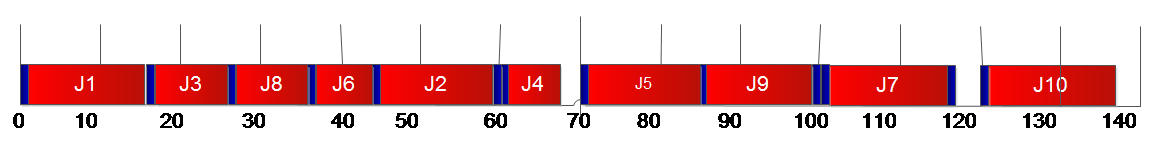
\includegraphics[scale=0.5]{Fig_1.png}
\\
Hình 1: Một lịch biểu tạo ra bởi kết hợp 2 heuristic HEU1 và HEU2.
\end{center}
Lịch biểu này có makespan là 137 và tổng độ trễ là 281.
\section{Giới thiệu giải thuật di truyền}
Giải thuật di truyền (hay giải thuật tiến hóa nói chung) là một trong những phát triển quan trọng của những nhà nghiên cứu về tính toán ứng dụng cuối thế kỷ trước trong việc giải xấp xỉ các bài toán tối ưu toàn cục. Việc khai thác nguyên lí tiến hóa như là một định hướng heuristics đã giúp cho giải thuật di truyền giải quyết hiệu quả các bài toán tối ưu (với các lời giải chấp nhận được) mà không cần sử dụng các điều kiện truyền thống (liên tục hay khả vi) như là điều kiện tiên quyết.\\\\
Một trong những đặc tính quan trọng của giải thuật di truyền là làm việc theo quần thể các giải pháp. Việc tìm kiếm bây giờ được thực hiện song song song trên nhiều điểm (multipoints).\\\\
Tuy nhiên, đây không phải là là thuật toán tìm kiếm đa điểm đơn thuần vì các điểm có tương tác với nhau theo nguyên lí tiến hóa tự nhiên. Trong ngữ cảnh sử dụng giải thuật di truyền, người ta có thể dùng khái niệm "cá thể" tương đương với khái niệm "giải pháp". Các bước cơ bản của giải thuật di truyền được mô tả như sau:
\begin{itemize}
\item
\textbf{Bước 1:} $t=0;$ Khởi tạo $P(t) = \{x_1,x_2,\ldots,x_N\}$, với $N$ là tổng số lượng cá thể.
\item
\textbf{Bước 2:} Tính giá trị các hàm mục tiêu cho $P(t)$.
\item
\textbf{Bước 3:} Tạo bể lai ghép $MP = se\{P(t)\}$ với $se$ là toán tử lựa chọn.
\item
\textbf{Bước 4:} Xác định $P'(t) = cr\{MP\}$, với $cr$ là toán tử lai ghép.
\item
\textbf{Bước 5:} Xác định $P"(t) = mu\{P'(t)\}$, với $mu$ là toán tử đột biến.
\item
\textbf{Bước 6:} Tính giá trị các hàm mục tiêu cho $P"(t)$.
\item
\textbf{Bước 7:} Xác định $P(t+1) = P"(t)$ và đặt $t = t+1$.
\item
\textbf{Bước 8:} Quay lại Bước 3, nếu điều kiện dừng chưa thỏa mãn.
\end{itemize}
\textbf{- Biểu diễn giải pháp:} Đây là một trong những công việc quan trọng trong thiết kế giải thuật di truyền, quyết định việc áp dụng các toán tử tiến hóa. Một trong những biểu diễn truyền thống của GA là biểu diễn nhị phân. Với phép biểu diễn này, giải pháp cho một bài toán được biểu diễn như là một vector bit, còn gọi là nhiễm sắc thể. Mỗi nhiễm sắc thể bao gồm nhiều gen, trong đó một gen đại diện cho một tham số thành phần của giải pháp. Một kiểu biểu diễn khác cũng thường dùng là biểu diễn số thực. Với phép biểu diễn này, các toán tử tiến hóa sẽ thực hiện trực tiếp trên các giá trị số thực (genes).\\
\textbf{- Lựa chọn:} Việc lựa chọn các cá thể được thực hiện khi cần một số cá thể để thực hiện sinh sản ra thế hệ sau. Mỗi cá thể có một giá trị thích nghi (fitness). Giá trị này được dùng để quyết định xem lựa chọn cá thể nào. Một số phương pháp lựa chọn thường dùng bao gồm:\\
\textit{+ Roulette wheel:} Dựa trên xác suất (tỷ lệ thuận với giá trị hàm thích nghi) để lựa chọn cá thể.\\
\textit{+ Giao đấu (nhị phân):} Chỉ định ngẫu nhiên 2 cá thể, sau đó chọn cá thể tốt hơn trong hai cá thể đó.\\
\textbf{- Lai ghép:} Toán tử lai ghép được áp dụng nhằm sinh ra các cá thể con mới từ các cá thể cha mẹ, thừa hưởng các đặc tính tốt từ cha mẹ. Trong ngữ cảnh tìm kiếm thì toán tử lai ghép thực hiện tìm kiếm xung quanh khu vực của các giải pháp biểu diển bởi các cá thể cha mẹ.\\
\textbf{- Đột biến:} Tương tự như lai ghép, đột biến cũng là toán tử mô phỏng hiện tượng đột biến trong sinh học. Kết quả của đột biến thường sinh ra các cá thể mới khác biệt so với cá thể cha mẹ. Trong ngữ cảnh tìm kiếm, toán tử đột biến nhằm đưa quá trình tìm kiếm ra khỏi khu vực cục bộ địa phương.
\section{Áp dụng giải thuật di truyền có sử dụng heuristic cho bài toán lập lịch đa mục tiêu}
Trong giải thuật di truyền, sau khi tạo ra quần thể, quần thể sẽ được tiến hóa qua nhiều thế hệ. Qua mỗi thế hệ, cá thể tốt nhất được lưu giữ cho quần thể tiếp theo. Sau khi tiến hóa xong, cá thể tốt nhất trong quần thể cuối cùng sẽ là phương án xếp lịch của bài toán. Thiết kế của giải thuật tập trung vào các vấn đề sau:\\
\textit{- Biểu diễn quần thể:} Biểu diễn các giá trị trong một nhiễm sắc thể, biểu diễn 1 cá thể của cá thể.\\
\textit{- Khởi tạo quần thể:} Khởi tạo quần thể ban đầu.\\
\textit{- Đánh giá cá thể:} Đánh giá độ tốt của cá thể.\\
\textit{- Các toán tử tiến hóa:} Định nghĩa phương pháp biến đổi nhiễm sắc thể trong quá trình tiến hóa.\\
\textit{- Cách thức tìm kiếm:} Tìm kiếm lời giải của bài toán bằng cách tìm cá thể tốt nhất của quần thể.
\subsection{Biểu diễn quần thể}
Biểu diễn là một vấn đề quan trọng đối với việc giải các bài toán lập lịch. Đối với bài toán này, chúng ta có thể sử dụng cách biểu diễn nguyên. Một giải pháp (lịch biểu hay biểu diễn của một cá thể trong quần thể) hoàn chỉnh bao gồm 4 thông tin sau: thứ tự các công việc không chu kỳ, thời gian hoàn thành (makespan), tổng độ trễ, giá trị mục tiêu dùng để đánh giá độ tốt của giải pháp được tính bằng công thức: \textbf{hệ số mục tiêu makespan * makespan + hệ số mục tiêu tổng độ trễ * tổng độ trễ\textit{}}. Ví dụ 1 giải pháp tạo ra bởi dùng kết hợp 2 heuristic HEU1 và HEU2 có thể được biểu diễn như sau (với hệ số mục tiêu makespan là 0.6 và hệ số mục tiêu tổng độ trễ là 0.4):
\begin{itemize}
\item
Thứ tự công việc: $J1 J3 J8 J6 J2 J4 J5 J9 J7 J10$
\item
Makespan: 137
\item
Tổng độ trễ : 281
\item
Giá trị mục tiêu: \textit{0.6*137 + 0.4*281 = 194.6}
\end{itemize}
\subsection{Khởi tạo quần thể}
Việc khởi tạo quần thể sẽ bao gồm việc khởi tạo các cá thể ban đầu cho quần thể. Số lượng các cá thể của quần thể sẽ được cho theo đầu vào của người dùng. Chúng ta sẽ tạo ra ngẫu nhiên những cá thể của quần thể. Trong quá trình tiến hóa của quần thể, chúng ta sẽ làm cho quần thể tốt hơn qua các thế hệ bằng cách thay thế những cá thể xấu nhất của quần thể bằng các cá thể con tốt hơn.
\subsection{Đánh giá cá thể}
Để đánh giá cá thể trong quần thể chúng ta căn cứ vào gía trị mục tiêu của mỗi giải pháp (cá thể). Cá thể tốt hơn sẽ có giá trị mục tiêu nhỏ hơn. Sau quá trình tiến hóa, chọn cá thể tốt nhất làm phương án cho bài toán.
\subsection{Các toán tử tiến hóa}
\begin{itemize}
\item
\textit{Toán tử chọn lọc:} Dùng để chọn ra những cá thể để lai ghép chúng với nhau sinh ra thế hệ con tiếp theo. Theo cách này chúng ta sẽ chọn ngẫu nhiên 2 cá thể trong quần thể để tham gia lai ghép.
\item
\textit{Toán tử lai ghép:} Có vai trò sống còn trong xác định hành vi của các giải thuật tiến hóa. Thông thường, hai cá thể được lựa chọn và các đặc tính của chúng được kết hợp để sinh ra hai cá thể con (offspring). Trong thiết kế này, chúng tôi sử dụng kỹ thuật lai hai điểm cắt (two-point crossover) tương tự như trong biểu diễn nhị phân. Với mỗi một lần thực hiện toán tử lai ghép, cần lựa chọn 2 điểm cắt, sau đó hoán đổi nội dung giữa hai điểm cắt. Ví dụ sau sẽ biểu diễn toán tử lai ghép được sử dụng:\\\\
\textit{Ví dụ:} Cho 2 cá thể: cá thể 1 có thứ tự các công việc như sau \textit{parent1:} $J1 J3 J2 J4 J5$, cá thể 2 có thứ tự các công việc \textit{parent2:} $J2 J5 J1 J3 J4$. Mỗi cá thể có 5 gen tương ứng với 5 công việc. Để lai ghép 2 cá thể này chúng ta sẽ chọn ra 2 điểm cắt, ví dụ 2 vị trí được chọn là 3 và 4. Tương ứng với 2 điểm cắt này đoạn gen được chọn lai ghép của cá thể 1 là $J2 J4$ và của cá thể 2 là $J1 J3$. Kết quả của việc lai ghép 2 cá thể này sẽ tạo ra 2 cá thể con mới là \textit{offspring1:} $J2 J4 J1 J3 J5$ và \textit{offspring2:} $J1 J5 J2 J4 J3$.\\\\
Sau khi đã lai ghép 2 cá thể để tạo ra 2 cá thể con, chúng ta sẽ áp dụng heuristic kết hợp cho 2 mục tiêu như ở ví dụ nêu trên. Mỗi cá thể con áp dụng heuristic sẽ tạo ra được 1 lịch biểu, vì vậy chúng ta sẽ có tổng cộng 2 cá thể con khi lai ghép 2 cá thể cha. Để có thể làm quần thể tốt hơn chúng ta sẽ xem xét lựa chọn 2 cá thể được đánh giá là xấu nhất trong quần thể hiện hành so sánh với 2 cá thể con được tạo ra. Từ 4 cá thể được xem xét chúng ta sẽ chọn ra 2 cá thể tốt nhất để đưa lại vào trong quần thể hiện hành. Cứ tiếp tục quá trình lai ghép chúng ta sẽ tiến dần làm cho quần thể mới được tạo ra càng ngày càng tốt hơn quần thể ban đầu.
\item
\textit{Toán tử đột biến:} Cũng như lai ghép, toán tử đột biến là một thành phần quan trọng trong thiết kế giải thuật tiến hóa. Khi thực hiện đột biến, một số giá trị gen của nhiễm sắc thể sẽ thay đổi ngẫu nhiên. Toán tử này hỗ trợ việc tạo ra một số đặc tính gen đã mất trong quá trình tiến hóa. Mỗi cá thể, chúng tôi chọn ngẫu nhiên một đoạn gen để thực hiện toán tử đột biến số nguyên.\\\\
\textit{Ví dụ:} Giả sử cá thể được chọn để đột biến như sau $J1 J3 J2 J4 J5$ và đoạn gen được chọn ngẫu nhiên để đột biến là $J1 J3$ sẽ được thay đổi với đoạn gen cũng được chọn ngẫu nhiên sau $J4 J5$. Cá thể mới sau khi đột biến sẽ có thứ tự là $J4 J5 J2 J1 J3$.\\\\
Tương tự như trong toán tử lai ghép, sau khi đột biến tạo ra thứ tự công việc mới chúng ta cũng áp dụng heuristic kết hợp để tạo ra 1 lịch biểu mới. Sau đó chúng ta sẽ thay thế cho lịch biểu (cá thể bị đột biến) để đưa lại vào trong quần thể.
\end{itemize}
\subsection{Chiến lược tìm kiếm}
Quần thể được tiến hóa qua nhiều thế hệ. Phần tử tốt nhất của thế hệ cuối cùng được chọn làm phương án của bài toán. Người dùng vẫn có thể thực hiện quá trình tiến hóa tiếp theo để chọn phương án phù hợp hơn. Qua mỗi lần tiến hóa, các cá thể ưu tú nhất nhằm giữ lại những thuộc tính tốt của từng thế hệ. Trong quần thể cuối cùng được tạo ra bởi giải thuật di truyền chúng ta sẽ tìm ra cá thể có giá trị mục tiêu nhỏ nhất là cá thể tốt nhất. Đây chính là lịch biểu cuối cùng của bài toán.
\section{Kết quả thực nghiệm}
Trong phần này chúng ta xem xét kết quả thực nghiệm khi chạy giải thuật di truyền có sử dụng heuristic. Chúng ta sẽ so sánh  giá trị mục tiêu của việc sử dụng giải thuật di truyền kết hợp 2 mục tiêu với giá trị mục tiêu khi sử dụng kết hợp 2 tập con thứ tự $J_{LPT}$ và $J_{EDF}$ như trong báo cáo [8]. Bên cạnh đó chúng ta cũng phải xem xét đến thời gian chạy giải thuật di truyền để xem xét cân bằng giữa việc tìm ra lời giải bài toán tốt hơn và thời gian cần thiết để tìm ra lời giải đó. Vì độ phức tạp của các heuristic là hàm tuyến tính nên thời gian chạy các heuristic gần như là ngay lập tức (không đáng kể). Đối với mỗi lần chạy giải thuật di truyền chúng ta sẽ xem xét chạy giải thuật trong một khoảng thời gian nhất định.\\\\
Đầu vào của thực nghiệm như sau:
\begin{itemize}
\item
Chu kỳ: 90, 100.
\item
Thời gian tính toán của công việc có chu kỳ: 40, 50.
\item
Số lượng các công việc không có chu kỳ: 100, 1000.
\item
Thời gian chạy giải thuật di truyền: 30 giây, 60 giây, 120 giây.
\item
Số lượng cá thể trong quần thể: 1000, 5000.
\item
Giá trị để xảy ra đột biến: 0.005, 0.01 (xảy ra đột biến khi chúng ta tạo ra một số ngẫu nhiên trong khoảng [0,1] có giá trị nhỏ hơn các giá trị trên).
\item
Hệ số mục tiêu của makespan là 0.6 và của tổng độ trễ là 0.4.
\end{itemize}
Kết quả thực nghiệm được cho bảng sau:\\\\
\begin{tabular}{|c|c|c|c|c|c|c|c|}
\hline
Cycle&Periodic&Aperiodic&Runtime(s)&Population&Mutate&Objective&GA Objective\\
\hline
90&40&100&30&1000&0.005&96951.8&55242.0\\
\hline
90&40&100&30&1000&0.01&96951.8&56123.2\\
\hline
90&40&100&30&5000&0.005&96951.8&59197.2\\
\hline
90&40&100&30&5000&0.01&96951.8&59299.4\\
\hline
90&40&100&60&1000&0.005&88243.6&36868.4\\
\hline
90&40&100&60&1000&0.01&88243.6&37434.0\\
\hline
90&40&100&60&5000&0.005&88243.6&36766.2\\
\hline
90&40&100&60&5000&0.01&88243.6&36424.2\\
\hline
90&40&100&120&1000&0.005&117758.4&55112.6\\
\hline
90&40&100&120&1000&0.01&117758.4&56122.2\\
\hline
90&40&100&120&5000&0.005&117758.4&55746.4\\
\hline
90&40&100&120&5000&0.01&117758.4&53516.4\\
\hline
90&40&1000&30&1000&0.005&11355712.2&9049719.0\\
\hline
90&40&1000&30&1000&0.01&11355712.2&9026400.6\\
\hline
90&40&1000&30&5000&0.005&11355712.2&9125558.2\\
\hline
90&40&1000&30&5000&0.01&11355712.2&9138448.2\\
\hline
90&40&1000&60&1000&0.005&11311075.6&8573027.6\\
\hline
90&40&1000&60&1000&0.01&11311075.6&8764387.2\\
\hline
90&40&1000&60&5000&0.005&11311075.6&8922606.2\\
\hline
90&40&1000&60&5000&0.01&11311075.6&8946820.6\\
\hline
90&40&1000&120&1000&0.005&10995668.8&8429130.8\\
\hline
90&40&1000&120&1000&0.01&10995668.8&8356571.4\\
\hline
90&40&1000&120&5000&0.005&10995668.8&8949635.4\\
\hline
90&40&1000&120&5000&0.01&10995668.8&8855115.8\\
\hline
90&50&100&30&1000&0.005&136454.4&75765.0\\
\hline
90&50&100&30&1000&0.01&136454.4&75811.4\\
\hline
90&50&100&30&5000&0.005&136454.4&80384.4\\
\hline
90&50&100&30&5000&0.01&136454.4&80668.4\\
\hline
\end{tabular}
\begin{tabular}{|c|c|c|c|c|c|c|c|}
\hline
Cycle&Periodic&Aperiodic&Runtime(s)&Population&Mutate&Objective&GA Objective\\
\hline
90&50&100&60&1000&0.005&121285.0&55025.0\\
\hline
90&50&100&60&1000&0.01&121285.0&54889.2\\
\hline
90&50&100&60&5000&0.005&121285.0&54494.4\\
\hline
90&50&100&60&5000&0.01&121285.0&54713.0\\
\hline
90&50&100&120&1000&0.005&131645.4&78540.2\\
\hline
90&50&100&120&1000&0.01&131645.4&78758.2\\
\hline
90&50&100&120&5000&0.005&131645.4&78381.8\\
\hline
90&50&100&120&5000&0.01&131645.4&78344.6\\
\hline
90&50&1000&30&1000&0.005&13269267.8&10787498.6\\
\hline
90&50&1000&30&1000&0.01&13269267.8&10656307.4\\
\hline
90&50&1000&30&5000&0.005&13269267.8&10822969.2\\
\hline
90&50&1000&30&5000&0.01&13269267.8&10854412.0\\
\hline
90&50&1000&60&1000&0.005&13107390.8&10277183.6\\
\hline
90&50&1000&60&1000&0.01&13107390.8&10294198.2\\
\hline
90&50&1000&60&5000&0.005&13107390.8&10679064.4\\
\hline
90&50&1000&60&5000&0.01&13107390.8&10486949.8\\
\hline
90&50&1000&120&1000&0.005&12932426.2&9600124.0\\
\hline
90&50&1000&120&1000&0.01&12932426.2&9590112.4\\
\hline
90&50&1000&120&5000&0.005&12932426.2&10357630.2\\
\hline
90&50&1000&120&5000&0.01&12932426.2&10241542.8\\
\hline
100&40&100&30&1000&0.005&97799.8&42373.2\\
\hline
100&40&100&30&1000&0.01&97799.8&41184.8\\
\hline
100&40&100&30&5000&0.005&97799.8&47006.8\\
\hline
100&40&100&30&5000&0.01&97799.8&48091.6\\
\hline
100&40&100&60&1000&0.005&110549.6&48542.6\\
\hline
100&40&100&60&1000&0.01&110549.6&49195.6\\
\hline
100&40&100&60&5000&0.005&110549.6&49502.0\\
\hline
100&40&100&60&5000&0.01&110549.6&48835.8\\
\hline
100&40&100&120&1000&0.005&125062.0&63538.0\\
\hline
100&40&100&120&1000&0.01&125062.0&63393.4\\
\hline
100&40&100&120&5000&0.005&125062.0&63704.4\\
\hline
100&40&100&120&5000&0.01&125062.0&62366.2\\
\hline
100&40&1000&30&1000&0.005&11443114.8&9156194.2\\
\hline
100&40&1000&30&1000&0.01&11443114.8&8970056.0\\
\hline
100&40&1000&30&5000&0.005&11443114.8&9163183.8\\
\hline
100&40&1000&30&5000&0.01&11443114.8&9215245.4\\
\hline
100&40&1000&60&1000&0.005&11284386.8&8503729.0\\
\hline
100&40&1000&60&1000&0.01&11284386.8&8519224.8\\
\hline
100&40&1000&60&5000&0.005&11284386.8&8796749.0\\
\hline
100&40&1000&60&5000&0.01&11284386.8&8834504.6\\
\hline
100&40&1000&120&1000&0.005&12479840.2&9274278.2\\
\hline
100&40&1000&120&1000&0.01&12479840.2&9220934.0\\
\hline
100&40&1000&120&5000&0.005&12479840.2&9761410.2\\
\hline
100&40&1000&120&5000&0.01&12479840.2&9745158.0\\
\hline
\end{tabular}
\begin{tabular}{|c|c|c|c|c|c|c|c|}
\hline
Cycle&Periodic&Aperiodic&Runtime(s)&Population&Mutate&Objective&GA Objective\\
\hline
100&50&100&30&1000&0.005&129661.8&56273.2\\
\hline
100&50&100&30&1000&0.01&129661.8&56644.0\\
\hline
100&50&100&30&5000&0.005&129661.8&60950.4\\
\hline
100&50&100&30&5000&0.01&129661.8&61317.2\\
\hline
100&50&100&60&1000&0.005&123100.4&54144.8\\
\hline
100&50&100&60&1000&0.01&123100.4&54394.6\\
\hline
100&50&100&60&5000&0.005&123100.4&54659.0\\
\hline
100&50&100&60&5000&0.01&123100.4&54743.8\\
\hline
100&50&100&120&1000&0.005&131978.4&63696.6\\
\hline
100&50&100&120&1000&0.01&131978.4&63389.0\\
\hline
100&50&100&120&5000&0.005&131978.4&63195.2\\
\hline
100&50&100&120&5000&0.01&131978.4&63609.8\\
\hline
100&50&1000&30&1000&0.005&13469694.6&10824622.8\\
\hline
100&50&1000&30&1000&0.01&13469694.6&10885202.6\\
\hline
100&50&1000&30&5000&0.005&13469694.6&10981492.8\\
\hline
100&50&1000&30&5000&0.01&13469694.6&10914048.0\\
\hline
100&50&1000&60&1000&0.005&13036761.6&10097350.0\\
\hline
100&50&1000&60&1000&0.01&13036761.6&10168857.6\\
\hline
100&50&1000&60&5000&0.005&13036761.6&10507793.4\\
\hline
100&50&1000&60&5000&0.01&13036761.6&10418251.6\\
\hline
100&50&1000&120&1000&0.005&13318776.0&10390838.6\\
\hline
100&50&1000&120&1000&0.01&13318776.0&10322684.6\\
\hline
100&50&1000&120&5000&0.005&13318776.0&10977562.6\\
\hline
100&50&1000&120&5000&0.01&13318776.0&10923943.8\\
\hline
\end{tabular}
\\\\
\hspace*{10mm}Bảng 1: Kết quả thực nghiệm.\\
\begin{itemize}
\item
\textit{Cycle:} Chu kỳ của công việc có chu kỳ.
\item
\textit{Periodic:} Thời gian tính toán của công việc có chu kỳ.
\item
\textit{Aperiodic:} Số lượng các công việc không có chu kỳ.
\item
\textit{RunTime:} Thời gian chạy giải thuật di truyền, tính bằng giây.
\item
\textit{Population:} Số lượng cá thể trong quần thể.
\item
\textit{Mutate:} Giá trị đột biến.
\item
\textit{Objective:} Giá trị mục tiêu khi sử dụng kết hợp 2 heuristic HEU1 và HEU2 như trong báo cáo [8].
\item
\textit{GA Objective:} Giá trị mục tiêu span khi chạy giải thuật di truyền kết hợp 2 heuristic HEU1 và HEU2.
\end{itemize}
\section{Kết luận}
Trong báo cáo này chúng ta đã giới thiệu bài toán lập lịch cho các công việc có chu kỳ và không có chu kỳ tối ưu đa mục tiêu thời gian hoàn thành và tổng độ trễ đồng thời nêu ra heuristic kết hợp để giải quyết bài toán trên. Heuristic đã có thể cho ra những lịch biểu đáp ứng được yêu cầu của bài toán. Tiếp theo chúng ta giới thiệu giải thuật di truyền và các nguyên lý của giải thuật. Sau đó áp dụng giải thuật di truyền đồng thời sử dụng áp dụng các heuristic ở trên để có thể tìm ra lịch biểu tốt hơn nữa trong một chừng mực cân bằng giữa độ tốt của kết quả tìm ra và thời gian chạy của giải thuật di truyền. Kết quả thực nghiệm cho thấy thời gian chạy giải thuật di truyền càng lâu thì càng tìm ra lời giải tốt hơn nhưng trong giới hạn, sau đó thì kết quả tìm ra không tốt hơn được nữa. Đồng thời trong khoảng thời gian đầu độ tốt của quần thể tăng nhanh và giảm dần sau đó.
\section{Tài liệu tham khảo}
1.	M.R. Garey, D.S. Johnson. Computers and Intractability: A Guide to the Theory of NP-Completeness. W.H. Freeman \& Company, San Francisco, 1979.\\
2.	R.L. Graham, E.L. Lawler, J.K. Lenstra, and A.H.G. Rinnooy Kan. Optimization and approximation in deterministic sequencing and scheduling: a survey. Annals of Discrete Mathematics 5, pp. 287–326, 1979.\\
3.	M. Ji, Y. He, T.C.E. Cheng. Single-machine scheduling with periodic maintenance to minimize makespan. Computer \& Operations Research 34, pp. 1764-1770, 2007.\\
4.	C.J. Liao, W.J. Chen. Single-machine scheduling with periodic maintenance and non-resumable jobs.\\
5.	S.N. Sivanandam, S.N. Deepa. Introduction to Genetic Algorithms.\\
6.	Huy NGUYEN VAN, Nguyen HUYNH TUONG, Hua Phung NGUYEN, Van Hoai TRAN, Slide "A Genetic Algorithm for Single-Machine Scheduling Problem with Splitable Jobs and Availability Constraints".\\
7.	Project VirtualLAB của Nguyễn Quyết Thắng, khoa Khoa Học và Kỹ Thuật Máy Tính, trường Đại Học Bách Khoa thành phố Hồ Chí Minh.\\
8.	Vũ Hà Thái, báo cáo "LẬP LỊCH CÁC CÔNG VIỆC CÓ CHU KỲ VÀ KHÔNG CHU KỲ TRONG MÔI TRƯỜNG MÁY ĐƠN ĐỂ TỐI ƯU HÓA ĐA MỤC TIÊU THỜI GIAN HOÀN THÀNH VÀ TỔNG ĐỘ TRỄ", khoa Khoa Học và Kỹ Thuật Máy Tính, trường Đại Học Bách Khoa thành phố Hồ Chí Minh.
\end{document}